\chapter{Project management techniques for small teams and startups}
\label{chap:techniques}

% Project management in the past
In the past project management was different. Not only because the formal discipline was mostly applied to the large projects lasting several years and costing millions of dollars, but also used a different approach, evolved from ancient military regimes, where relatively few people directed large number of others \cite{brandon}.

% Project definition, everything is a project, important skill
Project definition, as a temporary endeavour with a defined beginning and end \cite{chatfield}, undertaken to meet unique goals and objectives \cite{nokes} extends to the simple premise: everything is a project. For example important presentation or ``career development'' project, or even  employee development (each employee represents a single ``project'' in which it is required to keep track of performance and plan to help him or her develop). Pursuing goals makes project management techniques essential to get things done, and especially important for personal ones.

% Transition from general project management to modern software / product development methods
Downscaling project management to apply to the personal projects or small businesses required a different approach. In comparison to traditional ``waterfall'' model, which is inflexible and can potentially lead to a harmful consequences, a number of new methods emerged.

\section{Agile methods}

% Connect previous paragraph to ''agile'' introduction
A group of such methods, called ``Agile'' are a reaction to traditional ways of developing software and acknowledge the ``need for an alternative to documentation driven, heavyweight software development processes''.

The core of these methods consists of adaptive planning, evolutionary development and delivery, an iterative approach, and rapid and flexible response to change.

In 2001 the Manifesto for Agile Software Development \cite{agile-manifesto} was published to define the approach now known as agile software development. 

Some of the manifesto's authors formed the Agile Alliance (\url{http://www.agilealliance.org/}), a nonprofit organization that promotes software development according to the manifesto's principles.

% Manifesto itself
The Agile Manifesto:
\begin{quotation}
\begin{small}

We are uncovering better ways of developing software by doing it and helping others do it. Through this work we have come to value:

\begin{itemize}
\item Individuals and interactions over processes and tools
\item Working software over comprehensive documentation
\item Customer collaboration over contract negotiation
\item Responding to change over following a plan
\end{itemize}

That is, while there is value in the items on the right, we value the items on the left more.
\end{small}
\end{quotation}

% Explanation

Meaning, that self-organisation and motivation are important, working software will be more useful and welcome as a presentation for clients in meetings, collaboration leads to a better product, effectively tailored to the customer needs and quick changes allow higher quality of product.

\begin{figure}
	\centering
	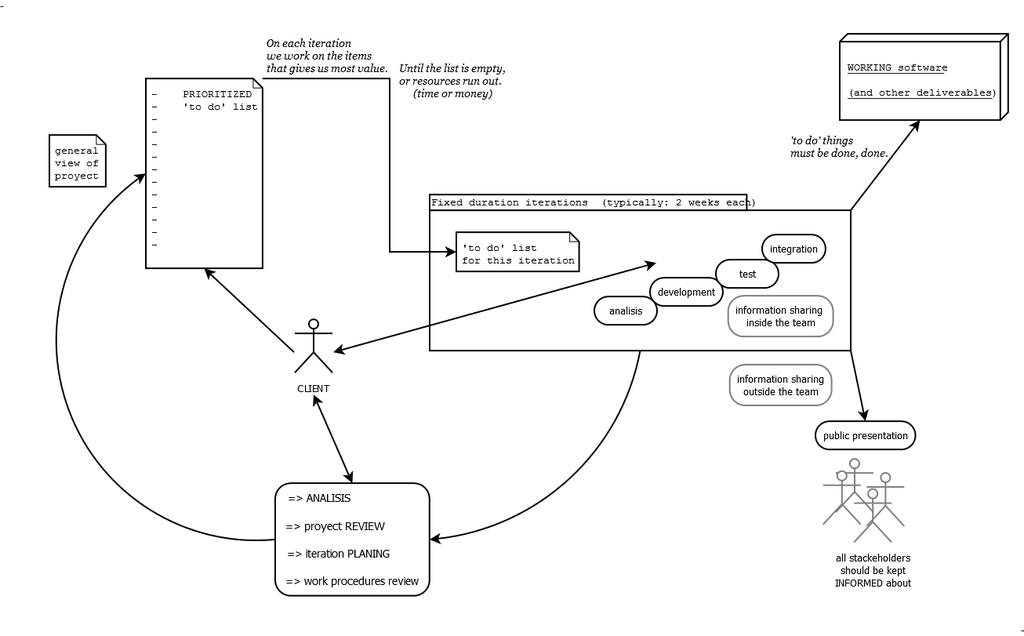
\includegraphics[width=0.8\textwidth]{resources/generic-diagram-agile.png}
	\caption[Generic agile diagram]{Generic agile diagram}
\end{figure}

% Prinicples

According to Kent Beck,\cite{beck} the Agile Manifesto is based on twelve principles:
\begin{compactenum}
\item Customer satisfaction by rapid delivery of useful software
\item Welcome changing requirements, even late in development
\item Working software is delivered frequently (weeks rather than months)
\item Working software is the principal measure of progress
\item Sustainable development, able to maintain a constant pace
\item Close, daily cooperation between business people and developers
\item Face-to-face conversation is the best form of communication (co-location)
\item Projects are built around motivated individuals, who should be trusted
\item Continuous attention to technical excellence and good design
\item Simplicity—the art of maximizing the amount of work not done—is essential
\item Self-organizing teams
\item Regular adaptation to changing circumstances
\end{compactenum}

% Where to use

Agile development is popular in a certain types of environment, including small teams. However a number of thing may negatively impact the success of an agile project:

\begin{compactenum}
\item Large-scale development efforts (\textgreater 20 developers), though scaling strategies \cite{ambler} and evidence of some large projects \cite{schaaf} have been described.
\item Distributed development efforts (non-colocated teams). Still there are examples of successful companies (37 Signals).
\item Forcing an agile process on a development team
\item Mission-critical systems where failure is not an option at any cost (e.g. software for air traffic control).
\end{compactenum}

Agile methods have been extensively used for development of software products and some of them use certain characteristics of software, such as object technologies. However, these techniques can be applied to the development of non-software products, such as computers, motor vehicles, medical devices, food, and clothing.

%\begin{longtable}{|p{0.25\textwidth}|p{0.25\textwidth}|p{0.25\textwidth}|}
%\caption{Suitability of different development methods}\label{tab:suitabilityddm} \\
%	\hline
%	\textbf{Agile} & \textbf{Plan-driven} & \textbf{Formal methods} \\
%	\hline
%	\endhead
%	Low criticality & High criticality & Extreme criticality \\
%	\hline
%	Senior developers & Junior developers & Senior developers \\
%	\hline
%	Requirements change often & Requirements do not change often & Limited requirements, limited features \\
%	\hline
%% дописать
%\end{longtable}


\section{Scrum}

One of the implementations of Agile philosophy is Scrum.

Authors describe Scrum, \cite{scrum-guide} as a framework within which people can address complex adaptive problems, while productively and creatively delivering products of the highest possible value.

\subsection{The Scrum team}

The Scrum Team consists of a Product Owner, the Development Team, and a Scrum Master. Scrum Teams are self-organising and cross-functional. Self-organising teams choose how best to accomplish their work, rather than being directed by others outside the team. Cross-functional teams have all competencies needed to accomplish the work without depending on others not part of the team. The team model in Scrum is designed to optimise flexibility, creativity, and productivity.

Scrum Teams deliver products iteratively and incrementally, maximising opportunities for feedback. Incremental deliveries of ``Done'' product ensure a potentially useful version of 
working product is always available.

\begin{figure}
	\centering
	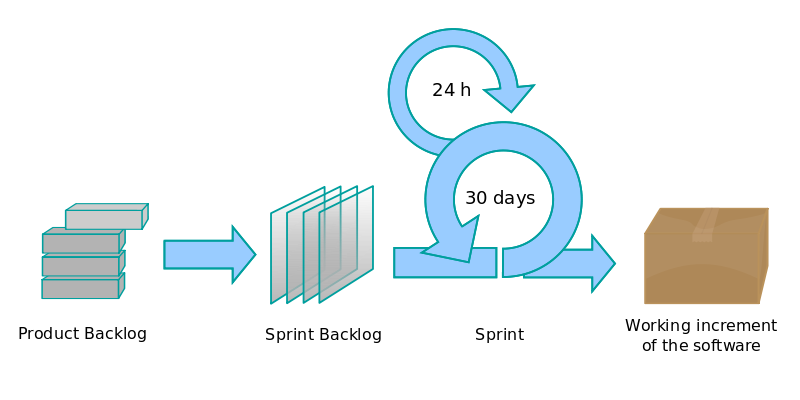
\includegraphics[width=0.8\textwidth]{resources/scrum-process.png}
	\caption[Scrum process]{Scrum process}
\end{figure}

\subsection{Scrum events}

Prescribed events are used in Scrum to create regularity and to minimise the need for meetings not defined in Scrum. Scrum uses time-boxed events, such that every event has a maximum duration. This ensures an appropriate amount of time is spent planning without allowing waste in the planning process.

Other than the Sprint itself, which is a container for all other events, each event in Scrum is a formal opportunity to inspect and adapt something. These events are specifically designed to enable critical transparency and inspection. Failure to include any of these events results in reduced transparency and is a lost opportunity to inspect and adapt.

\subsection{Scrum artifacts}

Scrum’s artifacts represent work or value in various ways that are useful in providing transparency and opportunities for inspection and adaptation. Artifacts defined by Scrum are specifically designed to maximise transparency of key information needed to ensure Scrum Teams are successful in delivering a ``Done'' Increment.

\section{RAD -- Rapid Application Development}

RAD is an integrated set of techniques, guidelines and tools that facilitate deploying a customer's software needs within a short period of time. This predefined timeframe is called a ``timebox''. The software product evolves during the RAD development process based on continued customer feedback. In addition, the whole software product is not delivered at once, but is delivered in pieces by order of business importance. \cite{gottesdiener}

\begin{figure}
	\centering
	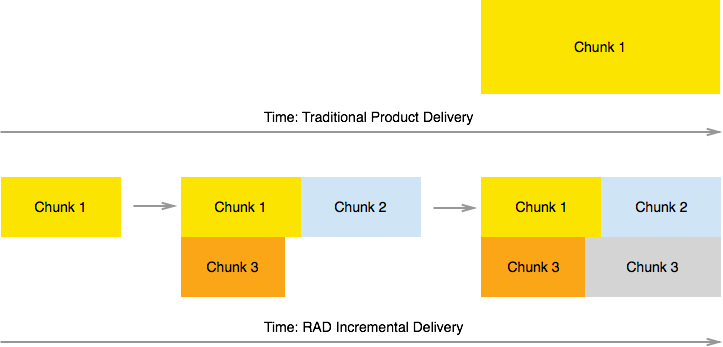
\includegraphics[width=0.8\textwidth]{resources/rad-incremental-delivery.png}
	\caption[RAD incremental delivery]{RAD incremental delivery}
\end{figure}

% bull's eye for RAD
% Timebox for each chunk


The RAD process defies a linear definition of steps carried out in a sequence. \cite{gottesdiener}

\subsection{Phases of RAD}

\begin{enumerate}
\item Requirements Planning phase -- combines elements of the system planning and systems analysis. During this stage, a definition of the project scope is completed along with some preliminary data/process analysis, risk assessment and estimating.

\item User design phase -- during this phase, users interact with systems analysts and develop models and prototypes that represent all system processes, inputs, and outputs. The RAD groups or subgroups typically use a combination of Joint Application Development (JAD) techniques and CASE tools to translate user needs into working models. User Design is a continuous interactive process that allows users to understand, modify, and eventually approve a working model of the system that meets their needs.

\begin{figure}
	\centering
	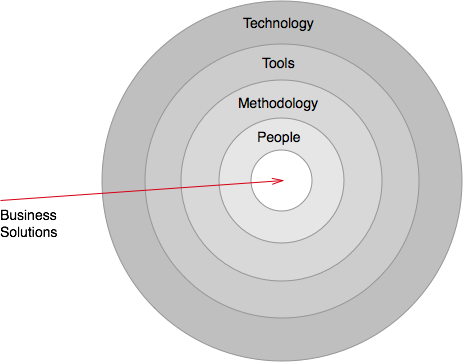
\includegraphics[width=0.6\textwidth]{resources/Rad-bulls-eye.png}
	\caption[Bull's eye for RAD]{Bull's eye for RAD, it should he the business problem, not the technology.}
\end{figure}

\item Construction phase -- focuses on program and application development task similar to the SDLC. In RAD, however, users continue to participate and can still suggest changes or improvements as actual screens or reports are developed. Its tasks are programming and application development, coding, unit-integration and system testing.

\begin{figure}
	\centering
	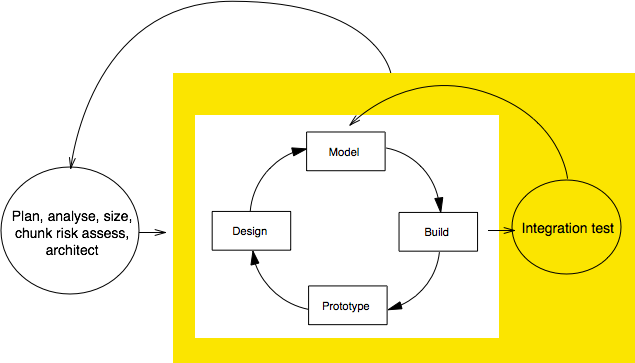
\includegraphics[width=0.6\textwidth]{resources/rad-timebox.png}
	\caption[RAD timeboxing]{RAD timeboxing for each ``chunk''. It forces project team to have a market product orientation}
\end{figure}


\item Cutover phase -- resembles the final tasks in the SDLC implementation phase, including data conversion, testing, changeover to the new system, and user training. Compared with traditional methods, the entire process is compressed. As a result, the new system is built, delivered, and placed in operation much sooner.
\end{enumerate}

In addition to using such techniques as timeboxing, chunking and customer-driven product delivery, RAD is based on the premise that software development is a discovery process.

% comparison table agile, lean, RAD, Scrum

\section{TDD -- Test-Driven Development}

Test-driven development (TDD) is a software development process that relies on the repetition of a very short development cycle: first the developer writes an (initially failing) automated test case that defines a desired improvement or new function, then produces the minimum amount of code to pass that test, and finally refactors the new code to acceptable standards. Kent Beck, who is credited with having developed or `rediscovered' the technique, stated in 2003 that TDD encourages simple designs and inspires confidence.

\subsection{TDD Cycle}

The TDD techniques is particularly interesting in terms of feedback, which helps to fail fast, be flexible and get a feeling of moving towards a goal. This is reached by using the following cycle.

\begin{figure}
	\centering
	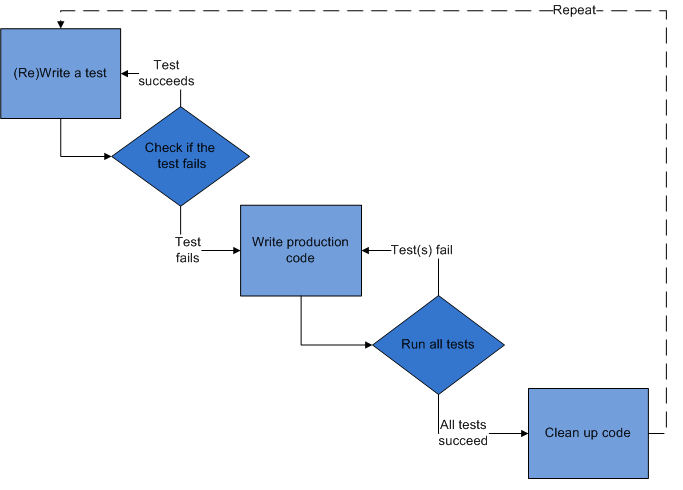
\includegraphics[width=0.8\textwidth]{resources/Test-driven_development.png}
	\caption[Test-Driven Development Cycle]{Test-Driven Development Cycle}
\end{figure}

\subsubsection{Add a test}

In test-driven development, each new feature begins with writing a test. This test must inevitably fail because it is written before the feature has been implemented. (If it does not fail, then either the proposed ``new'' feature already exists or the test is defective.) To write a test, the developer must clearly understand the feature's specification and requirements. The developer can accomplish this through use cases and user stories to cover the requirements and exception conditions, and can write the test in whatever testing framework is appropriate to the software environment. This could also be a modification of an existing test. This is a differentiating feature of test-driven development versus writing unit tests after the code is written: it makes the developer focus on the requirements before writing the code, a subtle but important difference.

\subsubsection{Run all tests and see if the new one fails}

This validates that the test harness is working correctly and that the new test does not mistakenly pass without requiring any new code. This step also tests the test itself, in the negative: it rules out the possibility that the new test always passes, and therefore is worthless. The new test should also fail for the expected reason. This increases confidence (though does not guarantee) that it is testing the right thing, and passes only in intended cases.

\subsubsection{Write some code}

The next step is to write some code that causes the test to pass. The new code written at this stage is not perfect, and may, for example, pass the test in an inelegant way. That is acceptable because later steps improve and hone it.

At this point, the only purpose of the written code is to pass the test; no further (and therefore untested) functionality should be predicted and 'allowed for' at any stage.

\subsubsection{Run the automated tests and see them succeed}

If all test cases now pass, the programmer can be confident that the code meets all the tested requirements. This is a good point from which to begin the final step of the cycle.

\subsubsection{Refactor code}

Now the code can be cleaned up as necessary. By re-running the test cases, the developer can be confident that code refactoring is not damaging any existing functionality. The concept of removing duplication is an important aspect of any software design. In this case, however, it also applies to removing any duplication between the test code and the production code—for example magic numbers or strings repeated in both to make the test pass in step 3.

\subsubsection{Repeat}

Starting with another new test, the cycle is then repeated to push forward the functionality. The size of the steps should always be small, with as few as 1 to 10 edits between each test run. If new code does not rapidly satisfy a new test, or other tests fail unexpectedly, the programmer should undo or revert in preference to excessive debugging. Continuous integration helps by providing revertible checkpoints. When using external libraries it is important not to make increments that are so small as to be effectively merely testing the library itself, unless there is some reason to believe that the library is buggy or is not sufficiently feature-complete to serve all the needs of the main program being written.

% Doesn't include other business goals. How we can project these on other aspects of business, not only development?


\section{FDD -- Feature-Driven Development}

FDD allows to manage projects at a very high level and apply other methodologies (such as TDD) at a lower level of abstraction. It is an iterative and incremental software development process, which primary focus is on being able to set estimates and schedules and to report on the status of a project, or its part. 

\subsection{Phases of FDD}

FDD consists of five basic activities. For accurate state reporting and keeping track of the software development project, milestones that mark the progress made on each feature are defined.

\subsubsection{Develop overall model}
The project started with a high-level walkthrough of the scope of the system and its context. Next, detailed domain walkthroughs were held for each modelling area. In support of each domain, walkthrough models were then composed by small groups, which were presented for peer review and discussion. One of the proposed models, or a merge of them, was selected which became the model for that particular domain area. Domain area models were merged into an overall model, and the overall model shape was adjusted along the way.

\subsubsection{Build feature list}

The knowledge that was gathered during the initial modelling was used to identify a list of features. This was done by functionally decomposing the domain into subject areas. Subject areas each contain business activities, the steps within each business activity formed the categorised feature list. Features in this respect were small pieces of client-valued functions expressed in the form ``<action> <result> <object>'', for example: `Calculate the total of a sale' or `Validate the password of a user'. Features should not take more than two weeks to complete, else they should be broken down into smaller pieces.

\subsubsection{Plan by feature}

After the feature list had been completed, the next step was to produce the development plan. Class ownership has been done by ordering and assigning features (or feature sets) as classes to chief programmers.

\subsubsection{Design by feature}

A design package was produced for each feature. A chief programmer selected a small group of features that are to be developed within two weeks. Together with the corresponding class owners, the chief programmer worked out detailed sequence diagrams for each feature and refines the overall model. Next, the class and method prologues are written and finally a design inspection is held.

\subsubsection{Build by feature}

After a successful design inspection a per feature activity to produce a completed client-valued function (feature) is being produced. The class owners develop the actual code for their classes. After a unit test and a successful code inspection, the completed feature is promoted to the main build.

\section{Lean}

Lean development is based on traditional lean principles, which are derived from the Japanese manufacturing industry. Generally ``Lean'' is a production practice that considers the expenditure of resources for any goal other than the creation of value for the end customer to be wasteful, and thus a target for elimination. Working from the perspective of the customer who consumes a product or service, ``value'' is defined as any action or process that a customer would be willing to pay for.

Lean development can be summarised by seven principles, very close in concept to lean manufacturing principles:
\begin{compactenum}
\item Eliminate waste
\item Amplify learning
\item Decide as late as possible
\item Deliver as fast as possible
\item Empower the team
\item Build integrity in
\item See the whole
\end{compactenum}

\subsection{Lean manufacturing principles}

\subsubsection{Eliminate waste}
Everything not adding value to the customer is considered to be waste (muda). This includes:
\begin{compactenum}
\item unnecessary code and functionality
\item delay in the software development process
\item unclear requirements
\item insufficient testing, leading to avoidable process repetition
\item bureaucracy
\item slow internal communication
\end{compactenum}

In order to be able to eliminate waste, one should be able to recognise it. If some activity could be bypassed or the result could be achieved without it, it is waste. Partially done coding eventually abandoned during the development process is waste. Extra processes and features not often used by customers are waste. Waiting for other activities, teams, processes is waste. Defects and lower quality are waste. Managerial overhead not producing real value is waste. A value stream mapping technique is used to distinguish and recognise waste. The second step is to point out sources of waste and eliminate them. The same should be done iteratively until even essential-seeming processes and procedures are liquidated.

\subsubsection{Amplify learning}

Software development is a continuous learning process with the additional challenge of development teams and end product sizes. The best approach for improving a software development environment is to amplify learning. The accumulation of defects should be prevented by running tests as soon as the code is written. Instead of adding more documentation or detailed planning, different ideas could be tried by writing code and building. The process of user requirements gathering could be simplified by presenting screens to the end-users and getting their input.

The learning process is sped up by usage of short iteration cycles -- each one coupled with refactoring and integration testing. Increasing feedback via short feedback sessions with customers helps when determining the current phase of development and adjusting efforts for future improvements. During those short sessions both customer representatives and the development team learn more about the domain problem and figure out possible solutions for further development. Thus the customers better understand their needs, based on the existing result of development efforts, and the developers learn how to better satisfy those needs. Another idea in the communication and learning process with a customer is set-based development -- this concentrates on communicating the constraints of the future solution and not the possible solutions, thus promoting the birth of the solution via dialogue with the customer.

\subsubsection{Decide as late as possible}

As software development is always associated with some uncertainty, better results should be achieved with an options-based approach, delaying decisions as much as possible until they can be made based on facts and not on uncertain assumptions and predictions. The more complex a system is, the more capacity for change should be built into it, thus enabling the delay of important and crucial commitments. The iterative approach promotes this principle -- the ability to adapt to changes and correct mistakes, which might be very costly if discovered after the release of the system.

An agile software development approach can move the building of options earlier for customers, thus delaying certain crucial decisions until customers have realised their needs better. This also allows later adaptation to changes and the prevention of costly earlier technology-bounded decisions. This does not mean that no planning should be involved -- on the contrary, planning activities should be concentrated on the different options and adapting to the current situation, as well as clarifying confusing situations by establishing patterns for rapid action. Evaluating different options is effective as soon as it is realised that they are not free, but provide the needed flexibility for late decision making.

\subsubsection{Deliver as fast as possible}

In the era of rapid technology evolution, it is not the biggest that survives, but the fastest. The sooner the end product is delivered without considerable defect, the sooner feedback can be received, and incorporated into the next iteration. The shorter the iterations, the better the learning and communication within the team. Without speed, decisions cannot be delayed. Speed assures the fulfilling of the customer's present needs and not what they required yesterday. This gives them the opportunity to delay making up their minds about what they really require until they gain better knowledge. Customers value rapid delivery of a quality product.

The just-in-time production ideology could be applied to software development, recognising its specific requirements and environment. This is achieved by presenting the needed result and letting the team organise itself and divide the tasks for accomplishing the needed result for a specific iteration. At the beginning, the customer provides the needed input. This could be simply presented in small cards or stories -- the developers estimate the time needed for the implementation of each card. Thus the work organisation changes into self-pulling system -- each morning during a stand-up meeting, each member of the team reviews what has been done yesterday, what is to be done today and tomorrow, and prompts for any inputs needed from colleagues or the customer. This requires transparency of the process, which is also beneficial for team communication. Another key idea in Toyota's Product Development System is set-based design. If a new brake system is needed for a car, for example, three teams may design solutions to the same problem. Each team learns about the problem space and designs a potential solution. As a solution is deemed unreasonable, it is cut. At the end of a period, the surviving designs are compared and one is chosen, perhaps with some modifications based on learning from the others -- a great example of deferring commitment until the last possible moment. Software decisions could also benefit from this practice to minimise the risk brought on by big up-front design.

\subsubsection{Empower the team}

There has been a traditional belief in most businesses about the decision-making in the organisation -- the managers tell the workers how to do their own job. In a Work-Out technique, the roles are turned -- the managers are taught how to listen to the developers, so they can explain better what actions might be taken, as well as provide suggestions for improvements. The lean approach favours the aphorism ``find good people and let them do their own job,'' encouraging progress, catching errors, and removing impediments, but not micro-managing.

Another mistaken belief has been the consideration of people as resources. People might be resources from the point of view of a statistical data sheet, but in software development, as well as any organisational business, people do need something more than just the list of tasks and the assurance that they will not be disturbed during the completion of the tasks. People need motivation and a higher purpose to work for -- purpose within the reachable reality, with the assurance that the team might choose its own commitments. The developers should be given access to the customer; the team leader should provide support and help in difficult situations, as well as ensure that skepticism does not ruin the team’s spirit.

\subsubsection{Build integrity in}

The customer needs to have an overall experience of the System -- this is the so-called perceived integrity: how it is being advertised, delivered, deployed, accessed, how intuitive its use is, price and how well it solves problems.

Conceptual integrity means that the system’s separate components work well together as a whole with balance between flexibility, maintainability, efficiency, and responsiveness. This could be achieved by understanding the problem domain and solving it at the same time, not sequentially. The needed information is received in small batch pieces -- not in one vast chunk with preferable face-to-face communication and not any written documentation. The information flow should be constant in both directions -- from customer to developers and back, thus avoiding the large stressful amount of information after long development in isolation.

One of the healthy ways towards integral architecture is refactoring. As more features are added to the original code base, the harder it becomes to add further improvements. Refactoring is about keeping simplicity, clarity, minimum amount of features in the code. Repetitions in the code are signs for bad code designs and should be avoided. The complete and automated building process should be accompanied by a complete and automated suite of developer and customer tests, having the same versioning, synchronization and semantics as the current state of the System. At the end the integrity should be verified with thorough testing, thus ensuring the System does what the customer expects it to. Automated tests are also considered part of the production process, and therefore if they do not add value they should be considered waste. Automated testing should not be a goal, but rather a means to an end, specifically the reduction of defects.

\subsubsection{See the whole}

Software systems nowadays are not simply the sum of their parts, but also the product of their interactions. Defects in software tend to accumulate during the development process -- by decomposing the big tasks into smaller tasks, and by standardising different stages of development, the root causes of defects should be found and eliminated. The larger the system, the more organisations that are involved in its development and the more parts are developed by different teams, the greater the importance of having well defined relationships between different vendors, in order to produce a system with smoothly interacting components. During a longer period of development, a stronger subcontractor network is far more beneficial than short-term profit optimising, which does not enable win-win relationships.

\section{Summarising agile, RAD and lean}

There is a common feature in all of the considered methodologies. According to table \ref{tab:prosconsitmet}, that is constructing a continuous feedback, which allows early failure and indicates whether a project goal is correct (or it should be adjusted) and a team progress. Each methodology provides its own level of abstraction and suggests tools to reduce chaos and uncertainty.

Comparing iterative methodologies to traditional waterfall model it is possible to say, that they appeared because of emergent projects with elements changing fast (goals, business processes, markets, etc.). Nonetheless traditional project management provides tools to cope with uncertainties, called PERT (section \ref{sec:pert}).

% Не нравится это предложение, нужно подумать
Ability to get instant feedback and adjust goals is defined by a natural human attribute as pursuing order in consciousness. This claim will be considered in section \ref{sec:flow} on page \pageref{sec:flow}.

\begin{longtable}{|p{0.15\textwidth}|p{0.35\textwidth}|p{0.35\textwidth}|}
\caption{Pros and cons of iterative methodics}\label{tab:prosconsitmet} \\
	\hline
	\textbf{Name} & \textbf{Pros} & \textbf{Cons} \\
	\hline
	\endhead
	Agile 
	& Minimises feature creep by developing in short intervals resulting in miniature software projects and releasing the product in mini-increments. 
	& Short iteration may add too little functionality, leading to significant delays in final iterations. Since Agile emphasises real-time communication (preferably face-to-face), using it is problematic for large multi-team distributed system development. Agile methods produce very little written documentation and require a significant amount of post-project documentation. \\
	\hline
	Lean 
	& Creates minimalist solutions and delivers less functionality earlier; per the policy that 80\% today is better than 100\% tomorrow. 
	& Product may lose its competitive edge because of insufficient core functionality and may exhibit poor overall quality. \\
	\hline
	RAD 
	& Promotes strong collaborative atmosphere and dynamic gathering of requirements. Business owner actively participates in prototyping, writing test cases and performing unit testing. 
	& Dependence on strong cohesive teams and individual commitment to the project. Decision-making relies on the feature functionality team and a communal decision-making process with lesser engineering authority. \\
	\hline
	Scrum 
	& Agile framework. Improved productivity in teams previously paralysed by heavy ``process'', ability to prioritise work, use of backlog for completing items in a series of short iterations or sprints, daily measured progress and communications. 
	& Reliance on facilitation by a master who may lack the political skills to remove impediments and deliver the sprint goal. Due to reliance on self-organising teams and rejection of traditional centralised ``process control'', internal power struggles can paralyse a team. \\
	\hline
\end{longtable}

\subsection{Program Evaluation and Review Technique}
\label{sec:pert}

% Relate to the previous sections

Let's also consider traditional ``waterfall'' methodology  statistical tool, designed to analyse and represent the tasks involved in completing a given project called PERT (Program Evaluation and Review Technique).

PERT was developed for the U.S. Navy Special Projects Office in 1957 to support the U.S. Navy's Polaris nuclear submarine project \cite{fazar}. It was able to incorporate uncertainty by making it possible to schedule a project while not knowing precisely the details and durations of all the activities. It is more of an event-oriented technique rather than start- and completion-oriented, and is used more in projects where time is the major factor rather than cost. It is applied to very large-scale, one-time, complex, non-routine infrastructure and Research and Development projects. An example of this was for the 1968 Winter Olympics in Grenoble which applied PERT from 1965 until the opening of the 1968 Games.


\begin{figure}
	\centering
	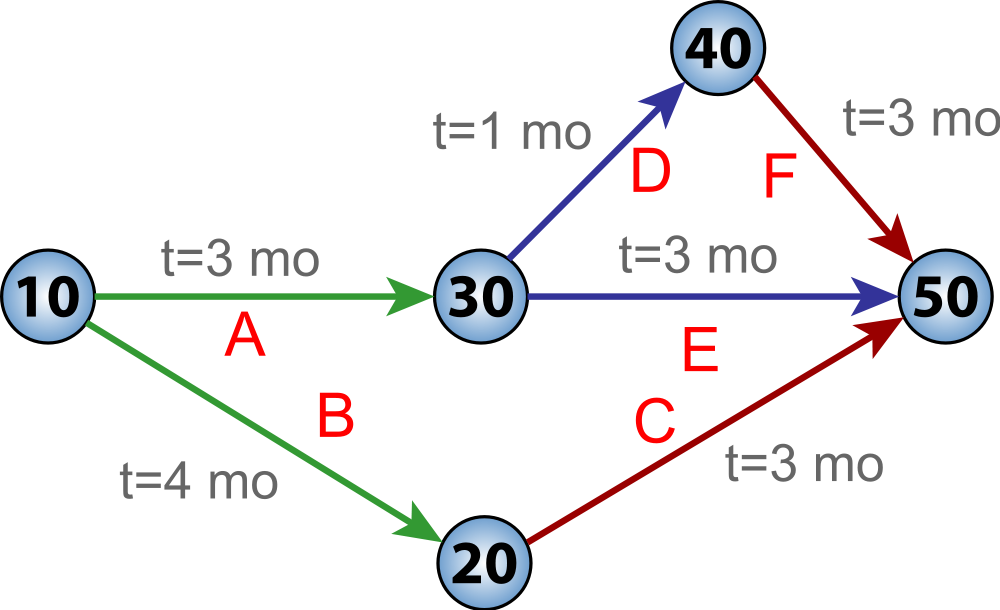
\includegraphics[width=0.6\textwidth]{resources/pert.png}
	\caption[PERT Chart]{PERT Chart}
\end{figure}

\subsubsection{Conventions}

\begin{compactitem}
% include pert illustration here
\item A PERT chart is a tool that facilitates decision making. The first draft of a PERT chart will number its events sequentially in 10s (10, 20, 30, etc.) to allow the later insertion of additional events.
\item Two consecutive events in a PERT chart are linked by activities, which are conventionally represented as arrows.
\item The events are presented in a logical sequence and no activity can commence until its immediately preceding event is completed.
\item The planner decides which milestones should be PERT events and also decides their ``proper'' sequence.
\item A PERT chart may have multiple pages with many sub-tasks.
\end{compactitem}

\subsubsection{Advantages}
\begin{compactitem}
\item PERT chart explicitly defines and makes visible dependencies (precedence relationships) between the work breakdown structure (commonly WBS) elements
\item PERT facilitates identification of the critical path and makes this visible
\item PERT facilitates identification of early start, late start, and slack for each activity,
\item PERT provides for potentially reduced project duration due to better understanding of dependencies leading to improved overlapping of activities and tasks where feasible.
\item The large amount of project data can be organised and presented in diagram for use in decision making.
\end{compactitem}

\subsubsection{Disadvantages}
\begin{compactitem}
\item There can be potentially hundreds or thousands of activities and individual dependency relationships
\item PERT is not easily scalable for smaller projects
\item The network charts tend to be large and unwieldy requiring several pages to print and requiring special size paper
\item The lack of a timeframe on most PERT/CPM charts makes it harder to show status although colours can help (e.g., specific colour for completed nodes)
\item When the PERT/CPM charts become unwieldy, they are no longer used to manage the project.
\end{compactitem}

\subsubsection{Uncertainty in project scheduling}

A real-life project will never execute exactly as it was planned due to uncertainty. It can be ambiguity resulting from subjective estimates that are prone to human errors or it can be variability arising from unexpected events or risks (which can drastically affect motivation of project participants, as the new information is in conflict with personal structure of goals). The main reason that PERT may provide inaccurate information about the project completion time is due to this schedule uncertainty. This inaccuracy is large enough to render such estimates as not helpful.

One possibility to maximise solution robustness is to include safety in the baseline schedule in order to absorb the anticipated disruptions. This is called proactive scheduling. A pure proactive scheduling is a utopia, incorporating safety in a baseline schedule that allows to cope with every possible disruption would lead to a baseline schedule with a very large make-span. A second approach, reactive scheduling, consists of defining a procedure to react to disruptions that cannot be absorbed by the baseline schedule.

Another approach incorporates Monte-Carlo analysis and simulates potential effects of schedule shifts.

\subsection{Tracking status of a project}

So, there is a technique to collect feedback in a large-scale projects. As any project could be considered as a system, it has different number of parts. As complexity of a system increases exponentially /cite{oconnor}, PERT tries to define relations and predict possible system states.

Use of iterative methods simplifies the system, and makes cause-and-effect relation clear.

Now team working on a project is able to collect necessary feedback in order to understand the state of a system. Thus it is possible to measure effectiveness (and make necessary adjustments to processes). But team members should be motivated in order to perform best.

\section{``Action Method'' application and concept behind}

This section describes an interesting technique, created by Behance company \cite{belsky}. It will be further used to construct an effectiveness guide.

The Action Method begins with a simple premise: everything is a project. Most creative people struggle to make progress in all of their projects, with the greatest challenge being the sheer number of projects before a person! But once everything has been classified as a project, it is possible to break each one down into its primary components: Action Steps, References, and Backburner Items.


\begin{figure}
	\centering
	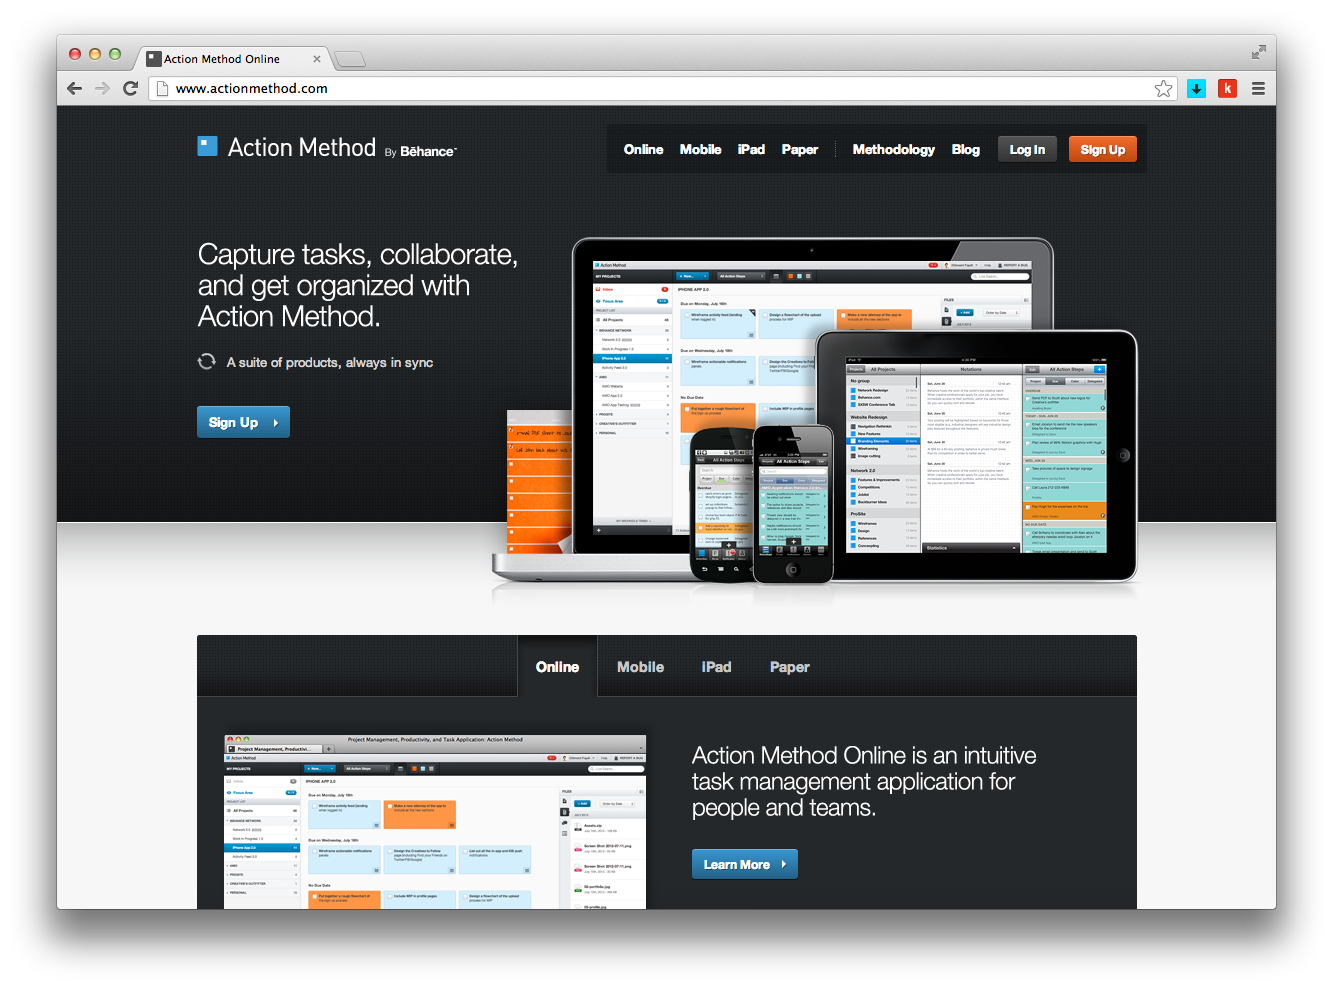
\includegraphics[width=0.8\textwidth]{resources/actionmethod.png}
	\caption[Action Method by Behance]{Action Method Landing Page by Behance}
\end{figure}

Every project in life can be reduced into these three primary components.

\subsection{Primary components of ``Action Method''}

\textbf{Action Steps}

Action steps are the specific, concrete tasks: redraft and send the memo, post the blog entry, pay the electricity bill, etc.

\textbf{References}

References are any project-related handouts, sketches, notes, meeting minutes, manuals, websites, or ongoing discussions to refer back to. It is important to note that references are not actionable—they are simply there for reference when focusing on any particular project.

\textbf{Backburner Items}

Backburner items -- things that are not actionable now but may be someday. Perhaps it is an idea for a client for which there is no budget yet. Or maybe it is something you intend to do in a particular project at an unforeseen time in the future.

Every project in life can be reduced into these three primary components.

Let’s consider a sample project for a client. Assume a folder with that client’s name on it. Inside the folder there is a lot of References -- a copy of the contract, notes from meetings, and background information on the client. The Action Steps (to-do list) could be written as a list, attached to the front of the folder. On a sheet stapled to the inside back cover of the folder, Backburner list could keep track of the non-actionable ideas that come up while working on the project.

With this hypothetical folder in mind, it is possible to imagine that the majority of focus would be on the Action Steps visible on the front cover. These Action Steps are always in plain view, while other parts accessible during the review phase.

Personal projects can also be broken down into the same three elements. The Action Method starts by considering everything with a project lens and then breaking it down.

\subsection{Action Steps in detail}

Action Steps are the most important components of projects. The actual outcome of any idea is dependent on the Actions Steps that are captured and then completed by you or delegated to someone else. Action Steps are to be revered and treated as sacred in any project. The more clear and concrete an Action Step is, the less friction a person will encounter trying to do it. If an Action Step is vague or complicated, a person will probably skip over it to others on the list that are more straightforward.

To avoid this, it is required to start each Action Step with a verb:
\begin{compactitem}
   \item Call programmer to discuss...
   \item Install new software for...
   \item Research the possibility of...
   \item Mock up a sample of the...
   \item Update XYZ document for...
\end{compactitem}

Verbs help to pull into Action Steps at first glance, efficiently indicating what type of action is required. For similar reasons, Action Steps should be kept short.

Ideas don’t reveal themselves only in meetings, and neither should Action Steps.

\textbf{An unowned Action Step will never be taken.}

Every Action Step must be owned by a single person. While some Action Steps may involve the input of different people, accountability must reside in one individual’s hands. Some people who lead teams or have assistants will capture Action Steps and delegate them to others. However, Action Step must still be owned by the person ultimately responsible.

\textbf{Every Action Step must be owned by a single person.}

The reason comes down to accountability. The practice of simply emailing someone a task to complete does not provide any assurance that it will be completed. For this reason, Action Steps that a person is ultimately responsible for should remain on your list until completed—even when a person have delegated them to others. Simply marking that the Action Step has been delegated and to whom is sufficient.

\textbf{Managerial Action Steps should be treated differently.}

Aside from the Action Steps that are personal, there are three other types of Action Steps one should keep in mind as the leader of a project. The first type is delegated Action Steps. The second type is ``Ensure Action Steps.'' Sometimes one will want to create an Action Step to ensure that something is completed properly in the future. Rather than being a nag to a  team, one can create an Action Step that starts with the word ``ensure.'' Creating ``Ensure Action Steps'' is a better alternative then sending numerous reminder emails to team members.

\textbf{The last type of managerial Action Step is the ``Awaiting'' Action Step.}

When one leaves a voicemail for someone, send a message to a potential customer, or respond to an email and clear it from the inbox, it is possible to forget to follow-up if the person fails to respond. So one should create an Action Step that starts with ``Awaiting''. In the online task manager one will set a target date for one week later. After a week passes, one will be reminded to follow up.

\textbf{Foster an action-oriented culture.}

A team needs an action-oriented culture to capitalise on creativity and effectiveness. It may feel a bit aggressive to ask people to capture an Action Step on paper, but fostering a culture in which such reminders are welcome helps ensure that Action Steps are not lost.

% Moving towards team-motivation

%\chapter{Project management without project manager}
%
%This chapter is about communication within a team, team motivational strategies. When should a team have a project manager (or should it)? Project manager role rotation. Team members roles in the project and its relation to the notion of ''Happiness''.
%
%\section{Collaboration tools and project management}
%
%\subsection{''Basecamp'' case.}
%Interface description. No intended workflow.
%
%\subsection{''Action method'' case.}
%Interface description. Intended workflow.
%
%\subsection{Section summary}
%
%\section{Team motivation strategies}
%
%\subsection{Goal commitment}
%
%R. Clark vision of team motivation strategies and what does goal commitment consists of.
%
%\subsection{M.C. on ''Flow''}
%
%\subsubsection{What is flow?}
%
%\subsubsection{Appication of flow to the business environment}
%
%\subsection{Section summary}


%\section{Another section}
%This section describes the section content.
%
%\subsection{``Subsection with quotes''}
%Items:
%\begin{itemize}
%	\item Item 1
%	\item Item 2 \& and sign.
%\end{itemize}
%
%Equation example:
%\begin{equation*}
%	\text{Luminance contrast} = \frac{\text{Luminance difference}}{\text{Average luminance}}
%\end{equation*}

% Different figures:
% \begin{figure}
% 	\centering
% 	\subfloat[Original image]{\label{fig:original}\includegraphics[width=0.3\textwidth]{resources/basic}}
% 	\hspace{0.01\textwidth}
% 	\subfloat[Brightness parameter set to 100, contrast parameter set to 0]{\label{fig:brightness_100}\includegraphics[width=0.3\textwidth]{resources/brightness_100}}
% 	\hspace{0.01\textwidth}
% 	\subfloat[Brightness parameter set to 0, contrast parameter set to 50]{\label{fig:contrast_50}\includegraphics[width=0.3\textwidth]{resources/contrast_50}}
% 	\\
% 	\subfloat[Histogram of \ref{fig:original}]{\includegraphics[width=0.3\textwidth]{resources/original_hist}}
% 	\hspace{0.01\textwidth}
% 	\subfloat[Histogram of \ref{fig:brightness_100}]{\includegraphics[width=0.3\textwidth]{resources/brightness_hist_100}}
% 	\hspace{0.01\textwidth}
% 	\subfloat[Histogram of \ref{fig:contrast_50}]{\includegraphics[width=0.3\textwidth]{resources/contrast_hist_50}}
% 	\caption{Effect of brightness/contrast tool application}
% 	\label{fig:brightness_contrast}
% \end{figure}